[64 v\textsuperscript{o}] manifesta consideranti ratio est. Esto Polus Arcticus\protect\index{Sachverzeichnis}{polus!arcticus} \textit{a} Antarcticus\protect\index{Sachverzeichnis}{polus!antarcticus} \textit{b}.
   % Bild aus satztechnischen Gruenden in 64r verschoben
   % \begin{wrapfigure}{l}{0.4\textwidth}          
   % 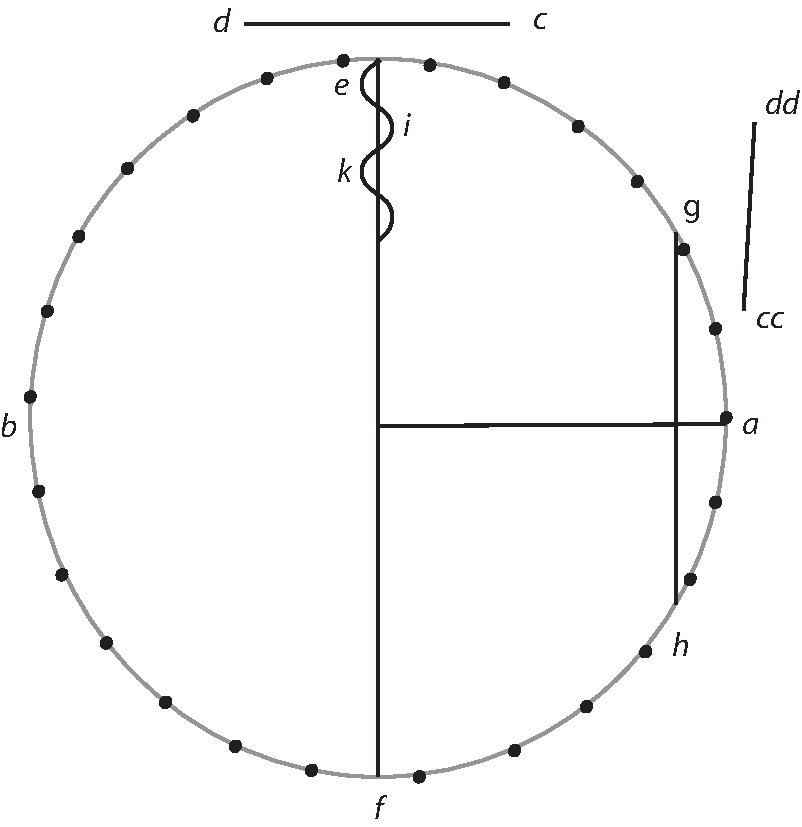
\includegraphics[width=0.4\textwidth]{images/35_15_6_64v}
   %\caption{Bildbeschreibung}
   %  \end{wrapfigure}
Acus magnetica\protect\index{Sachverzeichnis}{acus!magnetica} \textit{cd} sub linea aequinoctiali\protect\index{Sachverzeichnis}{linea!aequinoctialis} \edtext{\textit{ef}}{\lemma{}\Afootnote{\textit{ef} \textit{ erg.} \textit{ L }}} posita cujus extremitas \textit{c} arcticum\protect\index{Sachverzeichnis}{polus!arcticus}, at \textit{d} antarcticum polum \protect\index{Sachverzeichnis}{polus!antarcticus}respiciat. Manifestum est, cum aequalis sit conatus\protect\index{Sachverzeichnis}{conatus} \textit{d} versus \textit{b} et \textit{c} versus \textit{a} acum\protect\index{Sachverzeichnis}{acus!magnetica} sub \edtext{aequatore\protect\index{Sachverzeichnis}{aequator} \textit{ef}}{\lemma{sub}\Afootnote{ \textit{ (1) }\ linea \textit{ (2) }\ aequatore \textit{ef} \textit{ L}}} in aequilibrio\protect\index{Sachverzeichnis}{aequilibrium} ac proinde horizonti parallelam manere \edtext{ac proinde sub linea navigantibus, qui scilicet variis maeandris ut \textit{eik} lineam crebro secant, acum, ut a Lusitanis observatum est, perpetuo titubare}{\lemma{}\Afootnote{ac [...] titubare \textit{ erg.} \textit{ L}}}. At cis lineam inter \textit{e} et \textit{a} vel \textit{f} et \textit{a} seu sub parallelo\protect\index{Sachverzeichnis}{circulus parallelus} \textit{gh} praevalebit utique polus\protect\index{Sachverzeichnis}{polus} propinquior \textit{a} ac proinde illuc magis declinabit \edtext{acus\protect\index{Sachverzeichnis}{acus}}{\lemma{declinabit}\Afootnote{ \textit{ (1) }\ navis\protect\index{Sachverzeichnis}{navis|textit} \textit{ (2) }\ acus \textit{ L}}} contraria trans Lineam ratio est. \edtext{Idem Terrellae seu Magnetis in Globum tornati experimento confirmari potest}{\lemma{Idem}\Afootnote{ \textit{ (1) }\ experimento Terrellae magneticae\protect\index{Sachverzeichnis}{magnetica!terrella|textit} confirmari potest \textit{ (2) }\ Terrellae seu \textit{(a)}\ globi \textit{(b)}\ Magnetis [...] potest \textit{ L}}}, \edtext{cui acus imposita eodem plane modo}{\lemma{potest,}\Afootnote{ \textit{ (1) }\ ubi acus eodem plane modo \textit{ (2) }\ cui [...] modo \textit{ L}}} se disponit.\pend
   %\begin{center}          
   %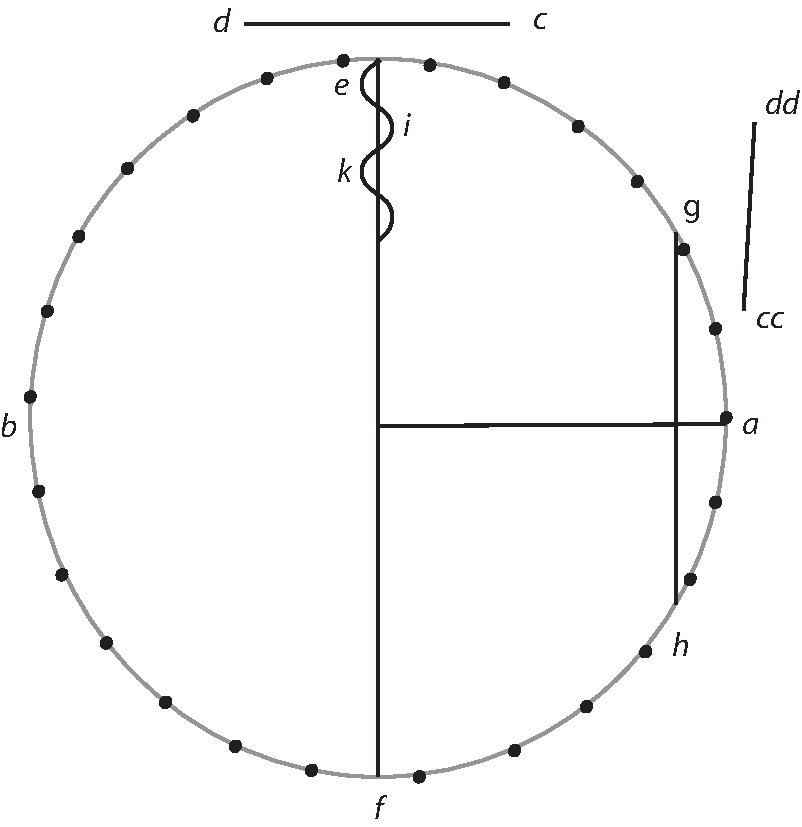
\includegraphics[width=0.7\textwidth]{images/35_15_6_64v}
   %\\\textit{[Fig. 1, tlw. Blindzeichnung]}
   %\end{center}
\pstart Et scripsit mihi aliquando R. P. Kircherus\protect\index{Namensregister}{\textso{Kircher} (Kircherus), Athanasius SJ 1602\textendash 1680}\edtext{}{\lemma{}\Afootnote{Kircherus \textbar\ cui caeteris certe \textit{ gestr.}\ \textbar\ novissimis \textit{ L}}} novissimis Patrum societatis in omnes Mundi plagas navigationibus plane extra dubium positam esse acus inclinatoriae\protect\index{Sachverzeichnis}{acus!inclinatoria} veritatem.\edtext{}{\lemma{veritatem.}\Bfootnote{Brief von A. Kircher am 23. Juni 1670 an Leibniz, \cite{00255}\textit{LSB} II, 1 N. 23.}} Quo posito ut ad certam \edtext{universalemque ab omni observatione coelesti et aeris injuria independentem}{\lemma{}\Afootnote{universalemque ab omni  \textbar\ observatione coelesti et \textit{ erg.}\ \textbar\ aeris injuria independentem \textit{ erg.} \textit{ L}}} Elevationis Poli\protect\index{Sachverzeichnis}{elevatio!poli} \edtext{investigationem}{\lemma{}\Afootnote{investigationem \textit{ erg.} \textit{ L}}} per \edtext{magnetem\protect\index{Sachverzeichnis}{magnes} perveniatur}{\lemma{magnetem}\Afootnote{ \textit{ (1) }\ universaliter sine ulla coeli observatione etiam in magnetis\protect\index{Sachverzeichnis}{magnes|textit} observationem \textit{ (2) }\ perveniatur \textit{ L}}}, duplex iniri via potest, altera Geometrica altera \edtext{Mechanica, ambaeque}{\lemma{Mechanica,}\Afootnote{ \textit{ (1) }\ utraque \textit{ (2) }\ ambaeque \textit{ L}}} inter se et experimentis sunt conjungendae. Quod Mechanicam attinet, tornandus est globus ex magnete\protect\index{Sachverzeichnis}{magnes} quantus optimus maximusque haberi potest, observandumque \edtext{quo in parallelo posita acus\protect\index{Sachverzeichnis}{acus} quo angulo}{\lemma{observandumque}\Afootnote{ \textit{ (1) }\ quos \textit{ (2) }\ quibus angulis \textit{ (3) }\ quo in parallelo posita acus \textit{(a)}\ quibus angulis \textit{(b)}\ quo angulo \textit{ L}}} inclinetur. Credibile est similem fore inclinationem acus\protect\index{Sachverzeichnis}{acus!inclinatoria} in tellure. \edtext{Via Geometrica est}{\lemma{tellure.}\Afootnote{ \textit{ (1) }\ Quod Viam Geometricam attinet \textit{ (2) }\ Via Geometrica est \textit{ L}}}, ut progressum inclinationis\protect\index{Sachverzeichnis}{inclinatio} crescentis decrescentisque observemus, ejusque \edtext{in regulas reductae}{\lemma{}\Afootnote{in regulas reductae \textit{ erg.} \textit{ L}}} tabulam si fieri potest ad minuta usque computatam condamus.\pend \pstart Experimentis autem sumtis repertum est, ipsum inclinationis\protect\index{Sachverzeichnis}{inclinatio} incrementum non esse uniforme, sed continue crescens. Hinc injecta mihi \textso{suspicio} est, \textso{inclinationes}\protect\index{Sachverzeichnis}{inclinatio}\textso{ esse sinubus proportionales.}\pend \pstart Notavi enim \edtext{plerosque naturae}{\lemma{enim}\Afootnote{ \textit{ (1) }\ naturam non angulos sed \textit{ (2) }\ plerosque naturae \textit{ L}}} effectus qui \edtext{angulis mutatis}{\lemma{qui}\Afootnote{ \textit{ (1) }\ pro angulorum ea ratione \textit{ (2) }\ angulis mutatis \textit{ L}}} variantur, non angulis sed sinubus \edtext{tangentibus, secantibusve}{\lemma{}\Afootnote{tangentibus, secantibusve \textit{ erg.} \textit{ L}}}, esse proportionales ita ictuum\protect\index{Sachverzeichnis}{ictus} obliquorum quantitas, et corporis in plano inclinato descendentis gravitas\protect\index{Sachverzeichnis}{gravitas} est ad gravitatem\protect\index{Sachverzeichnis}{gravitas} aut vim recta ferientis aut descendentis, \edtext{in}{\lemma{descendentis,}\Afootnote{ \textit{ (1) }\ ut \textit{ (2) }\ in \textit{ L}}} reciproca ratione secantis anguli inclinationis\protect\index{Sachverzeichnis}{inclinatio} ad radium.\pend \pstart Refractiones\protect\index{Sachverzeichnis}{refractio} quoque non ab angulis, sed sinubus pendere, nunc apud plerosque confirmatur. Idem de pendulorum\protect\index{Sachverzeichnis}{pendulum} vibrationibus in confesso est, et Illustris vir, Robertus Moraeus\protect\index{Namensregister}{\textso{Moray} (Moraeus), Robert 1608\textendash 1673} suspicatus est, etiam 